\documentclass{article}

\usepackage{amsmath,amssymb}
\usepackage{tikz}
\usepackage{pgfplots}
\usepackage{xcolor}
\usepackage[left=2.1cm,right=3.1cm,bottom=3cm,footskip=0.75cm,headsep=0.5cm]{geometry}
\usepackage{enumerate}
\usepackage{enumitem}
\usepackage{marvosym}
\usepackage{tabularx}
\usepackage{parskip}

\usepackage{listings}
\definecolor{lightlightgray}{rgb}{0.95,0.95,0.95}
\definecolor{lila}{rgb}{0.8,0,0.8}
\definecolor{mygray}{rgb}{0.5,0.5,0.5}
\definecolor{mygreen}{rgb}{0,0.8,0.26}
%\lstdefinestyle{java} {language=java}
\lstset{language=R,
	basicstyle=\ttfamily,
	keywordstyle=\color{lila},
	commentstyle=\color{lightgray},
	stringstyle=\color{mygreen}\ttfamily,
	backgroundcolor=\color{white},
	showstringspaces=false,
	numbers=left,
	numbersep=10pt,
	numberstyle=\color{mygray}\ttfamily,
	identifierstyle=\color{blue},
	xleftmargin=.1\textwidth, 
	%xrightmargin=.1\textwidth,
	escapechar=§,
	%literate={\t}{{\ }}1
	breaklines=true,
	postbreak=\mbox{\space}
}

\usepackage[colorlinks = true, linkcolor = blue, urlcolor  = blue, citecolor = blue, anchorcolor = blue]{hyperref}
\usepackage[utf8]{inputenc}

\renewcommand*{\arraystretch}{1.4}

\newcolumntype{L}[1]{>{\raggedright\arraybackslash}p{#1}}
\newcolumntype{R}[1]{>{\raggedleft\arraybackslash}p{#1}}
\newcolumntype{C}[1]{>{\centering\let\newline\\\arraybackslash\hspace{0pt}}m{#1}}

\newcommand{\E}{\mathbb{E}}
\DeclareMathOperator{\rk}{rk}
\DeclareMathOperator{\Var}{Var}
\DeclareMathOperator{\Cov}{Cov}

\title{\textbf{Kryptografie und -analyse, Zusammenfassung Vorlesung 8}}
\author{\textsc{Henry Haustein}}
\date{}

\begin{document}
	\maketitle
	
	\section*{Warum und wie kann CBC zur Authentikation verwendet werden? Welche Schwachstelle ist bekannt?}
	Verkettung der Schlüsseltextblöcke macht Manipulationen erkennbar, weil sich die Veränderung bis zum Ende durchzieht. Eine Schwachstelle ist existenzielles Brechen: Durch Manipulation des vorherigen Schlüsseltextes können einzelne Bytes des aktuelles Klartextes verändert werden. Die Veränderung fällt ab dem nächsten Schlüsseltext auf. Das kann mit CBC-MAC verhindert werden, allerdings gibt es dort eine andere Schwachstelle namens \textit{Length-Extension}: Ein Angreifer kann aus zwei gültigen Nachricht-MAC-Paaren einen gültigen MAC für eine neue Nachricht (die Konkatenation der beiden Nachrichten) erzeugen. Zwei Modifikationen können diesen Angriff verhindern: Jeder Nachricht kann die Nachrichtenlänge vorangestellt werden oder der MAC-Block wird zusätzlich mit einem zweiten Schlüssel verschlüsselt.
	
	Ein interessantes Youtube-Video dazu (behandelt allerdings CFB, der obige Angriff funktioniert aber fast genau so): \url{https://www.youtube.com/watch?v=i-2UgCDdhpM&t=822s}
	
	\section*{Wie funktioniert der Countermode?}
	Zur Verschlüsselung wird ein Initialisierungsvektor $IV$ mit dem Schlüssel $k$ verschlüsselt und so ein Zwischenschlüssel produziert. Dieser wird im Anschluss mittels einer XOR-Operation mit dem Klartext kombiniert. Daraus entsteht der Geheimtext.
	\begin{center}
		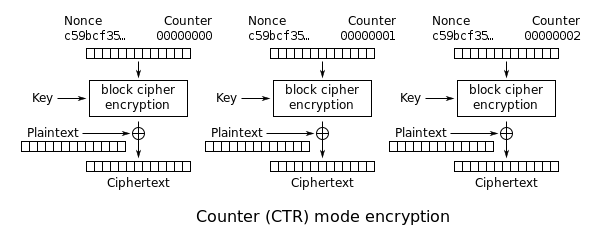
\includegraphics[scale=0.7]{CTR}
	\end{center}
	
	\section*{Wie wirken sich bei dieser Betriebsart Fehler bzw. Manipulationen während der Übertragung aus?}
	Fehler und Manipulationen fallen im aktuellen Block auf, falls ein Block gelöscht wird, geht die gesamte Synchronisation verloren.
	
	\section*{Warum darf der Zähler bei Verwendung desselben Schlüssels nur einmal verwendet werden?}
	Das erzeugt die selbe Folge von Schlüsseln und damit wird der selbe Plaintext zum selben Ciphertext.
	
	\section*{Welche Elemente gehören zu $\mathbb{Z}_n$, $\mathbb{Z}_n^\ast$ bzw. $\mathbb{Z}_p$, $\mathbb{Z}_p^\ast$?}
	$\mathbb{Z}_n = \{0,1,...,n-1\}$, $\mathbb{Z}_n^\ast = \{\text{teilerfremde Zahlen zu } n\}$, wenn $n$ prim, dann $\mathbb{Z}_n^\ast = \{1,2,...,n-1\}$
	
	\section*{Wie wird die Anzahl der Elemente dieser Gruppen bestimmt ($n = p\cdot q$; $p, q$ prim)?}
	$\mathbb{Z}_n$ hat $n$ Elemente, $\vert\mathbb{Z}_n^\ast\vert = \Phi(n) = \Phi(p\cdot q) = (p-1)(q-1)$
	
	\section*{Wie werden multiplikative Inverse bestimmt?}
	Erweiterter euklidischer Algorithmus: EEA($a$, $n$) $\Rightarrow$ $ua + vn = 1$ $\Rightarrow$ $u = a^{-1} \mod n$
	
	\section*{Wie können Primzahlen erzeugt werden?}
	Probabilistischer Test nach Rabin-Miller: Falls $p$ prim, dann $\forall a\in\mathbb{Z}_p^\ast: a^{\frac{p-1}{2}} \equiv \pm 1 \mod p$. Falls $p$ nicht prim, dann gilt dies höchstens für $\frac{1}{4}$ der möglichen $a$.
	
	\section*{Was versteht man unter einer zyklischen Gruppe? Was unter Generator?}
	Alle Elemente einer Gruppe $G$ lassen sich durch einen Generator $g\in G$ "generieren" durch Potenzieren: $G = \{g^0, g^1, ...\} = \langle g\rangle$
	
\end{document}